\section{Anexos}
\subsection{Modelo Físico}
\begin{center}
	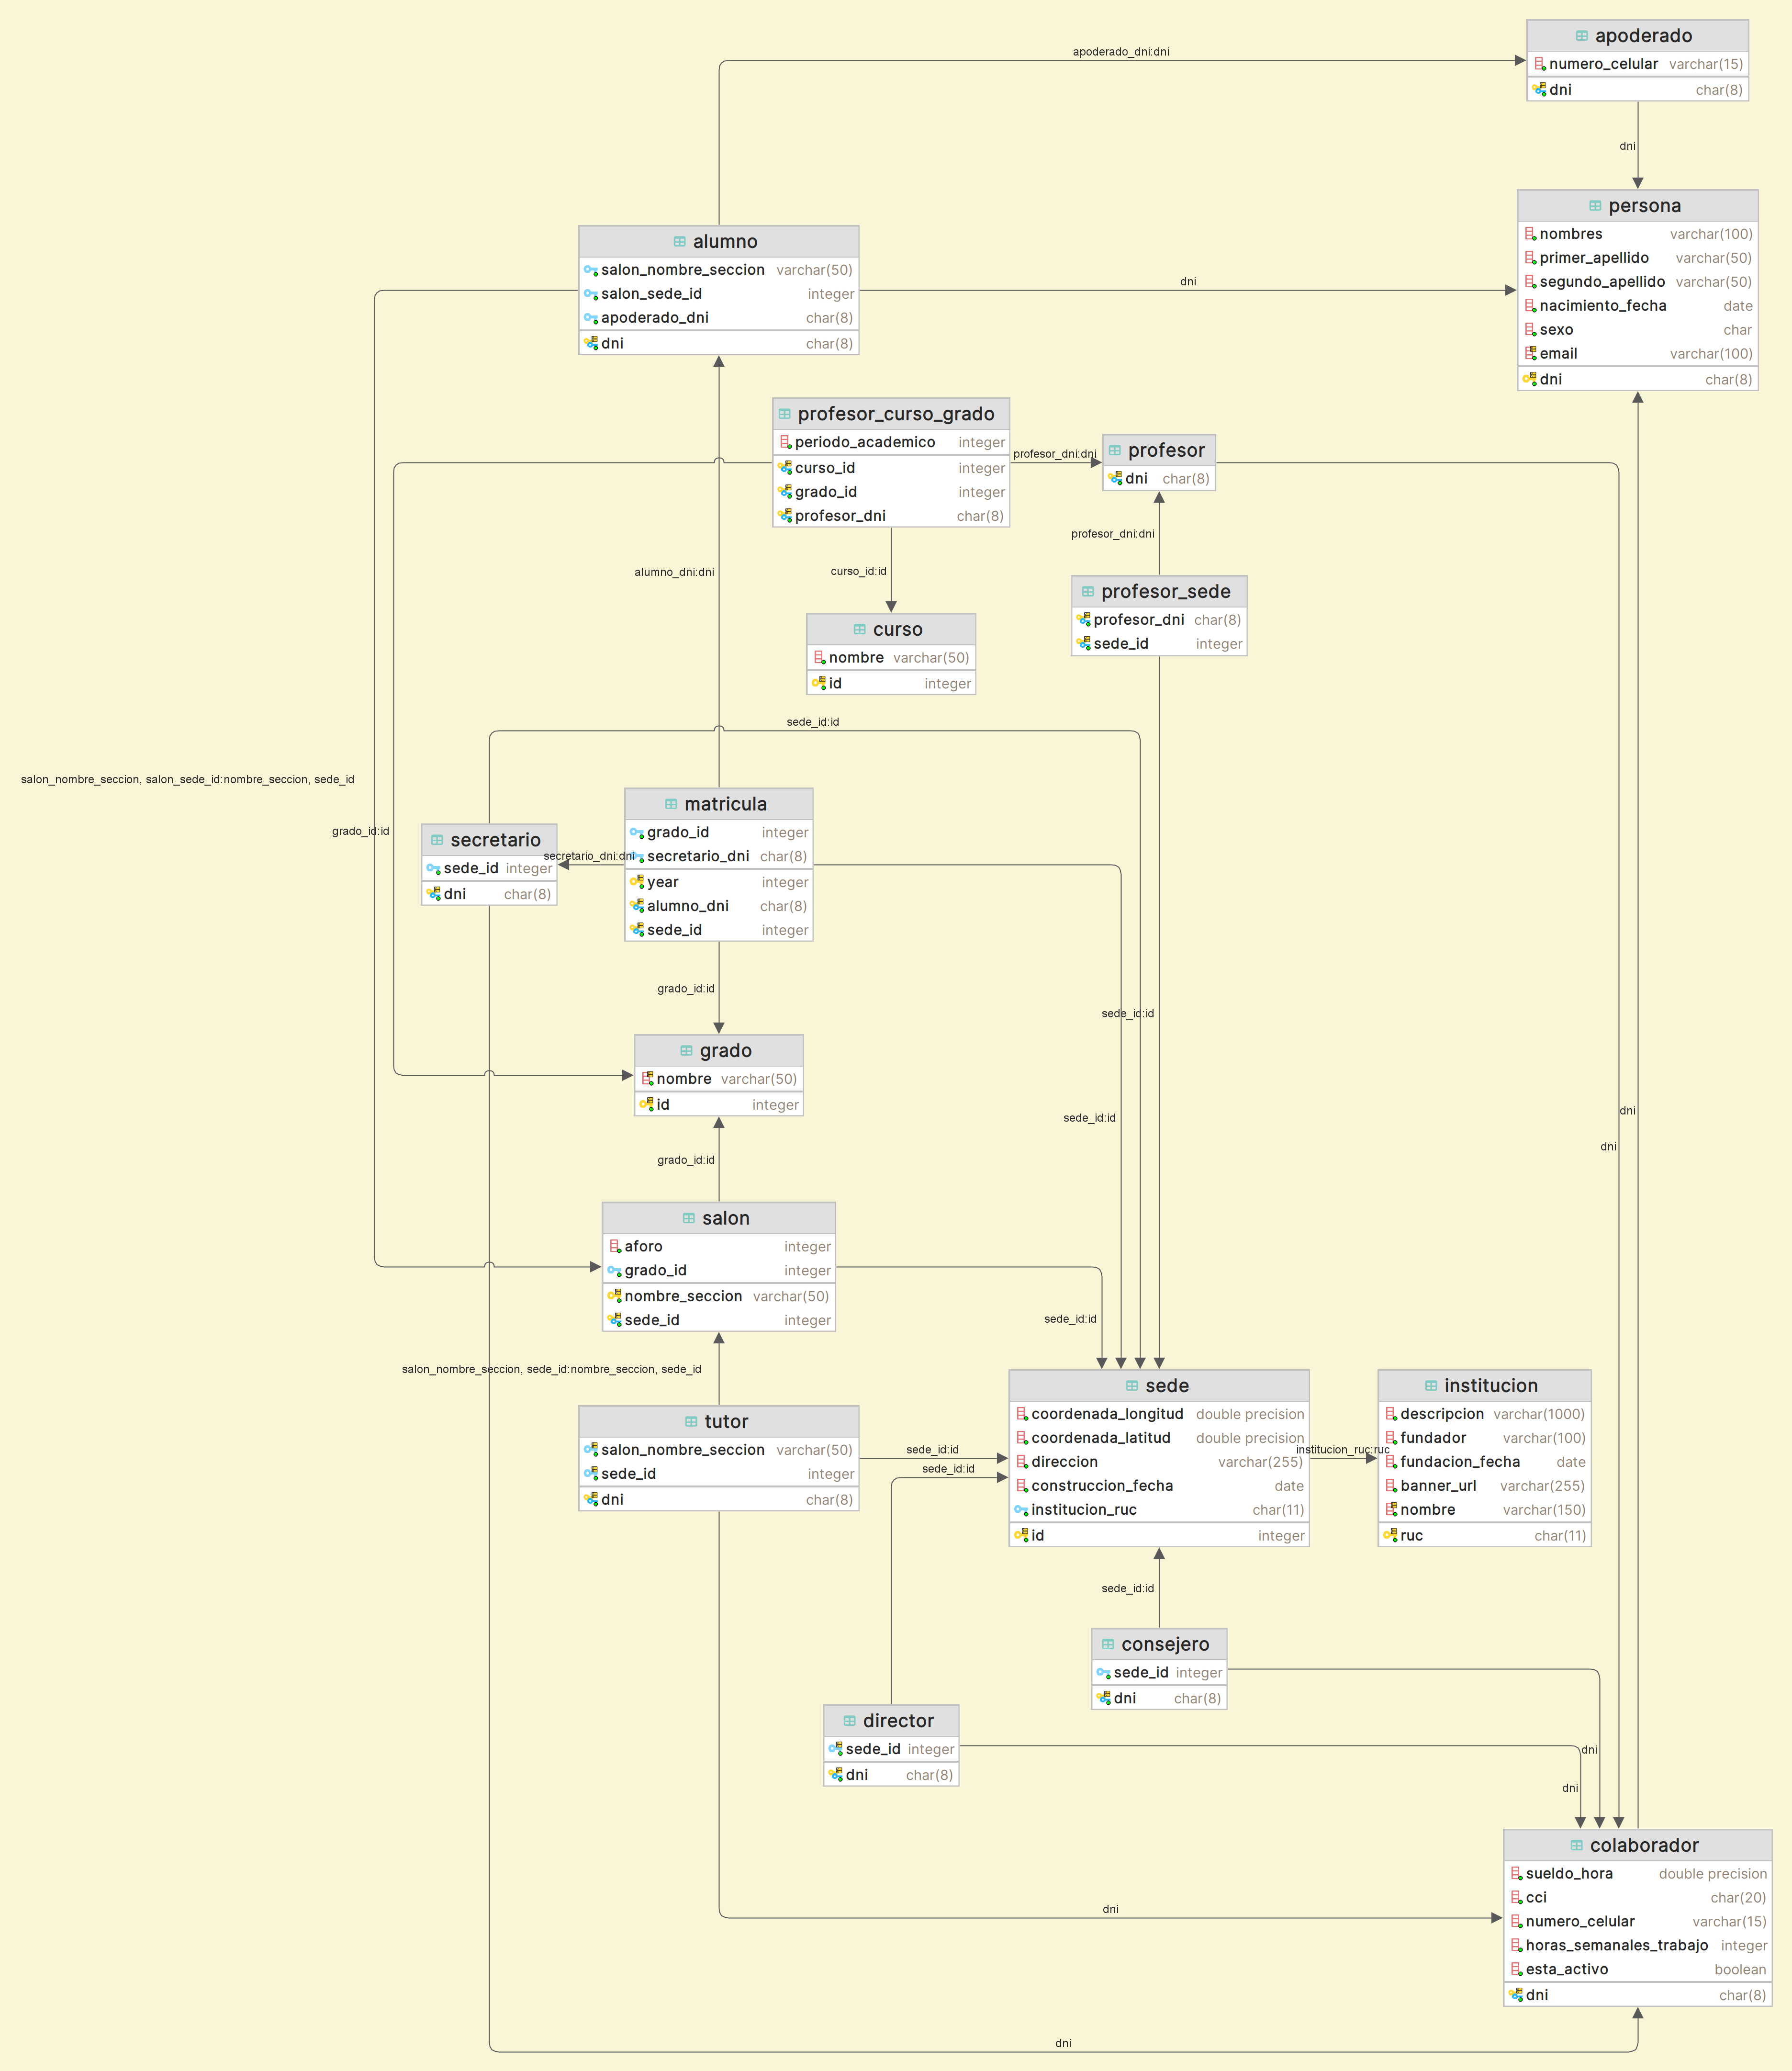
\includegraphics[width=\linewidth, height=0.75\textheight, keepaspectratio]{figures/modelo_fisico.png}
\end{center}
\subsection{Repositorios de GitHub}
\subsubsection{Repositorio del informe en LaTeX}{
	Este informe se ha realizado en LaTeX con el apoyo de GitHub, aprovechando sus herramientas de control de versiones y colaboración. La plataforma ha permitido documentar y gestionar cada etapa del proyecto con precisión. Para más detalles, acceda al repositorio en el siguiente enlace: \link{https://github.com/AlejandroEN/Database-I-Project-LaTex}{GitHub Repositorio}.
}
\subsubsection{Repositorio del código en SQL}{
	Los contenidos del proyecto, incluidos el código SQL, el script de Python y los archivos CSV, se encuentran disponibles en otro repositorio de GitHub. Para más detalles, acceda al repositorio en el siguiente enlace: \link{https://github.com/AlejandroEN/Database-I-Project-Code}{GitHub Repositorio}.
}
\subsubsection{Repositorio para el front-end}
Los contenidos del frontend creado para el proyecto están disponibles en el siguiente enlace: \link{https://github.com/AlejandroEN/Database-I-Project-Frontend}{GitHub Repositorio}.
\subsection{Videos de experimentación}
\subsubsection{Consulta 1}
\begin{itemize}
	\item{\link{https://drive.google.com/file/d/1G6OM4pp-3xyTvn61H--6IS_XM8IY5r9Y/view?usp=drive_link}{Sin índices}}
	\item{\link{https://drive.google.com/file/d/1PIcvrEYvBltJCNQ3aT1Mw-3fVKul6ZF7/view?usp=drive_link}{Con índices por defecto}}
	\item{\link{https://drive.google.com/file/d/1Wq7pbkbU5-_EUVC_Qv5p91xKB4gqvnJg/view?usp=drive_link}{Con índices por defecto más índices personalizados}}
\end{itemize}
\subsubsection{Consulta 2}
\begin{itemize}
	\item{\link{https://drive.google.com/file/d/1MM1AwEC-DH_eJeznwzYpQitviGYUi5pc/view?usp=drive_link}{Sin índices}}
	\item{\link{https://drive.google.com/file/d/1YAjI4YJ9u9ZD81UBYiR_kSDgV5RDfJAJ/view?usp=drive_link}{Con índices por defecto}}
	\item{\link{https://drive.google.com/file/d/16mElSCN6Zkx0KVM7f2qu_xNKIKmU2ui0/view?usp=drive_link}{Con índices por defecto más índices personalizados}}
\end{itemize}
\subsubsection{Consulta 3}
\begin{itemize}
	\item{\link{https://drive.google.com/file/d/1F6jeoqpubWSvGTXQOKCm5BVJsAo3rnO6/view?usp=drive_link}{Sin índices}}
	\item{\link{https://drive.google.com/file/d/1AgnL8Z3CL18vB3-PS9tncTY-1QJVyCRd/view?usp=drive_link}{Con índices por defecto}}
	\item{\link{https://drive.google.com/file/d/1fa3fXZATm_HrQGIlS0w_1TQo3g1SDgrg/view?usp=drive_link}{Con índices por defecto más índices personalizados}}
\end{itemize}
\subsection{Pregunta extra}
¿Cuál sería la complejidad operacional si escalamos los datos por encima del millón?, realice una comparativa respecto a la cantidad de datos del párrafo anterior. ¿Es suficiente la arquitectura Cliente-Servidor para procesar millones de datos?

Para manejar eficientemente millones de datos, es fundamental optimizar la estructura de índices, particionar tablas, utilizar almacenamiento en caché y considerar bases de datos no relacionales (NoSQL). Sistemas como MongoDB y Cassandra son gestores de bases de datos no relacionales que facilitan la gestión de grandes volúmenes de datos y proporcionan flexibilidad en el modelado de datos. Por otro lado, la arquitectura Cliente-Servidor es suficiente si se optimiza adecuadamente, permite escalabilidad horizontal, implementa balanceadores de carga y mitiga cuellos de botella en la red, CPU y disco. Una arquitectura distribuida puede ser necesaria para gestionar eficientemente las operaciones a gran escala.